
\setsecnumdepth{section}

\chapter{Eigenanalysis}
\label{ch:eigen}

The title of this chapter alone is enough to make one's blood run cold. You
might be thinking, ``even if I could pronounce this, would I want to?''

In German, the root \textit{eigen} (pronounced EYE-gun) means something like
``one's own, inherent thing.'' As we'll see, in studying the eigenvectors and
eigenvalues of a matrix -- a process called eigen-analysis -- we're examining
its deepest, innermost properties. We're peering deep within all the flesh to
see its skeleton. And it turns out this is the key to the most profound
understanding of what a given matrix is and does.

Just look at all the nifty words we'll learn:

\begin{compactitem}
\item \textbf{eigenvector}
\item \textbf{eigenvalue}
\item \textbf{eigendecomposition}
\item \textbf{eigenbasis}
\end{compactitem}

These are all involved in the \textbf{eigenanalysis} of a matrix.

\section{The resonant frequency}

\index{resonant frequency}
\index{frequency, resonant}

We could come at this subject in a bunch of different ways, but let me start
with the first thing that clicked for me when I learned it. At the time, I was
reminded of the phenomenon of a ``resonant frequency'' that some systems
exhibit.

\index{playground}
\index{swing}

You'll remember this effect if you've ever been on a playground swing. When
somebody pushes you (or when you pump your legs to ``push'' yourself) you have
to do it at the right time and at the right pace. The swing has a natural
frequency of oscillation, and it resists being pushed faster or slower than
that. If you find you're swinging from back to front every two seconds, you'll
have to pump your legs every two seconds. Period. Even if you have thighs like
Dwayne Johnson, trying to pump once every 1.5 seconds --  or even furiously at
5 times a second -- will do you no good. Timing it so you pump your legs at
exactly the swing's resonant frequency is the only way to go higher and higher.

\begin{center}
\label{tacoma}
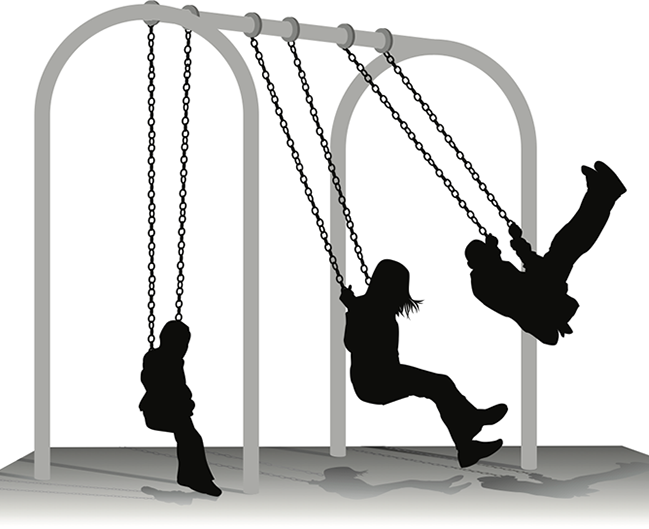
\includegraphics[width=0.45\textwidth]{swing.png}
\quad
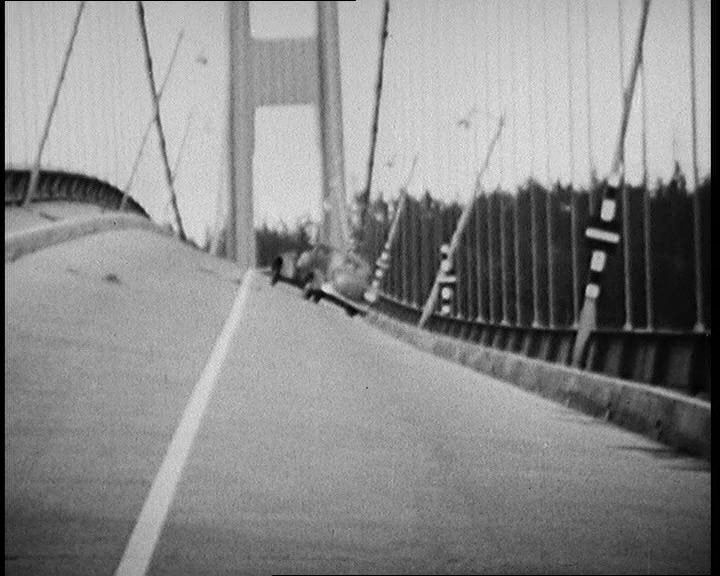
\includegraphics[width=0.45\textwidth]{tacoma.jpg}
\end{center}

\index{Tacoma Narrows Bridge}
\index{bridge}
\index{Slinky}

There are other famous examples of the resonant frequency phenomenon. Perhaps
you've heard of the Tacoma Narrows Bridge (if you've never seen it, check out
the video on
\href{https://www.youtube.com/watch?v=j-zczJXSxnw}{\underline{YouTube}}). It
was a beautiful double-lane suspension bridge in Washington State that crossed
the Puget Sound -- at the time, the third-largest suspension bridge in the
world. Incredibly, on November 7th, 1940, it began to wobble with increasing
intensity as crosswinds dangerously amplified its internal structural
vibrations. It looked like a 3,000-foot-long undulating Slinky.\footnote{The
classic ``Slinky'' toy, by the way, is another example of a system that has a
resonant frequency. You can't make it go down the stairs any faster or slower
than it wants to go.} Moments later, the concrete cracked and split and the
entire bridge completely collapsed and fell into the water. Luckily, drivers
had wisely stopped crossing it minutes before, and the only actual casualty was
a cocker spaniel.

The reasons for the Tacoma Bridge catastrophe are a bit complex, but a key
contributing factor was that a very specific rate of oscillation -- a ``sweet
spot,'' though it was hardly sweet for those involved -- caused the
fluctuations to build on each other instead of being dampened. It's as if the
Tacoma Bridge \textit{wanted} to vibrate at a certain frequency, just like a
playground swing has an intrinsic rhythm that the child can't speed up or slow
down.

\index{guitar}
\index{piano}
\index{middle C}

Yet another example: every non-percussive musical instrument. A piano or guitar
string tuned to middle~C has a certain length and tension, which causes it to
resist vibrations at any frequency other than exactly 262 per second. Thus,
when you strike it, only the 262~Hz\footnote{``Hz,'' pronounced ``hertz,'' is a
unit meaning ``cycles (backs-and-forths) per second.'' Every musical note is
defined by a particular frequency. The lowest key on the piano is 27.5~Hz, and
the highest is 4,186~Hz.} tone gains any traction, and the instrument sounds a
clear, pure note.

\begin{center}
\label{slinky}
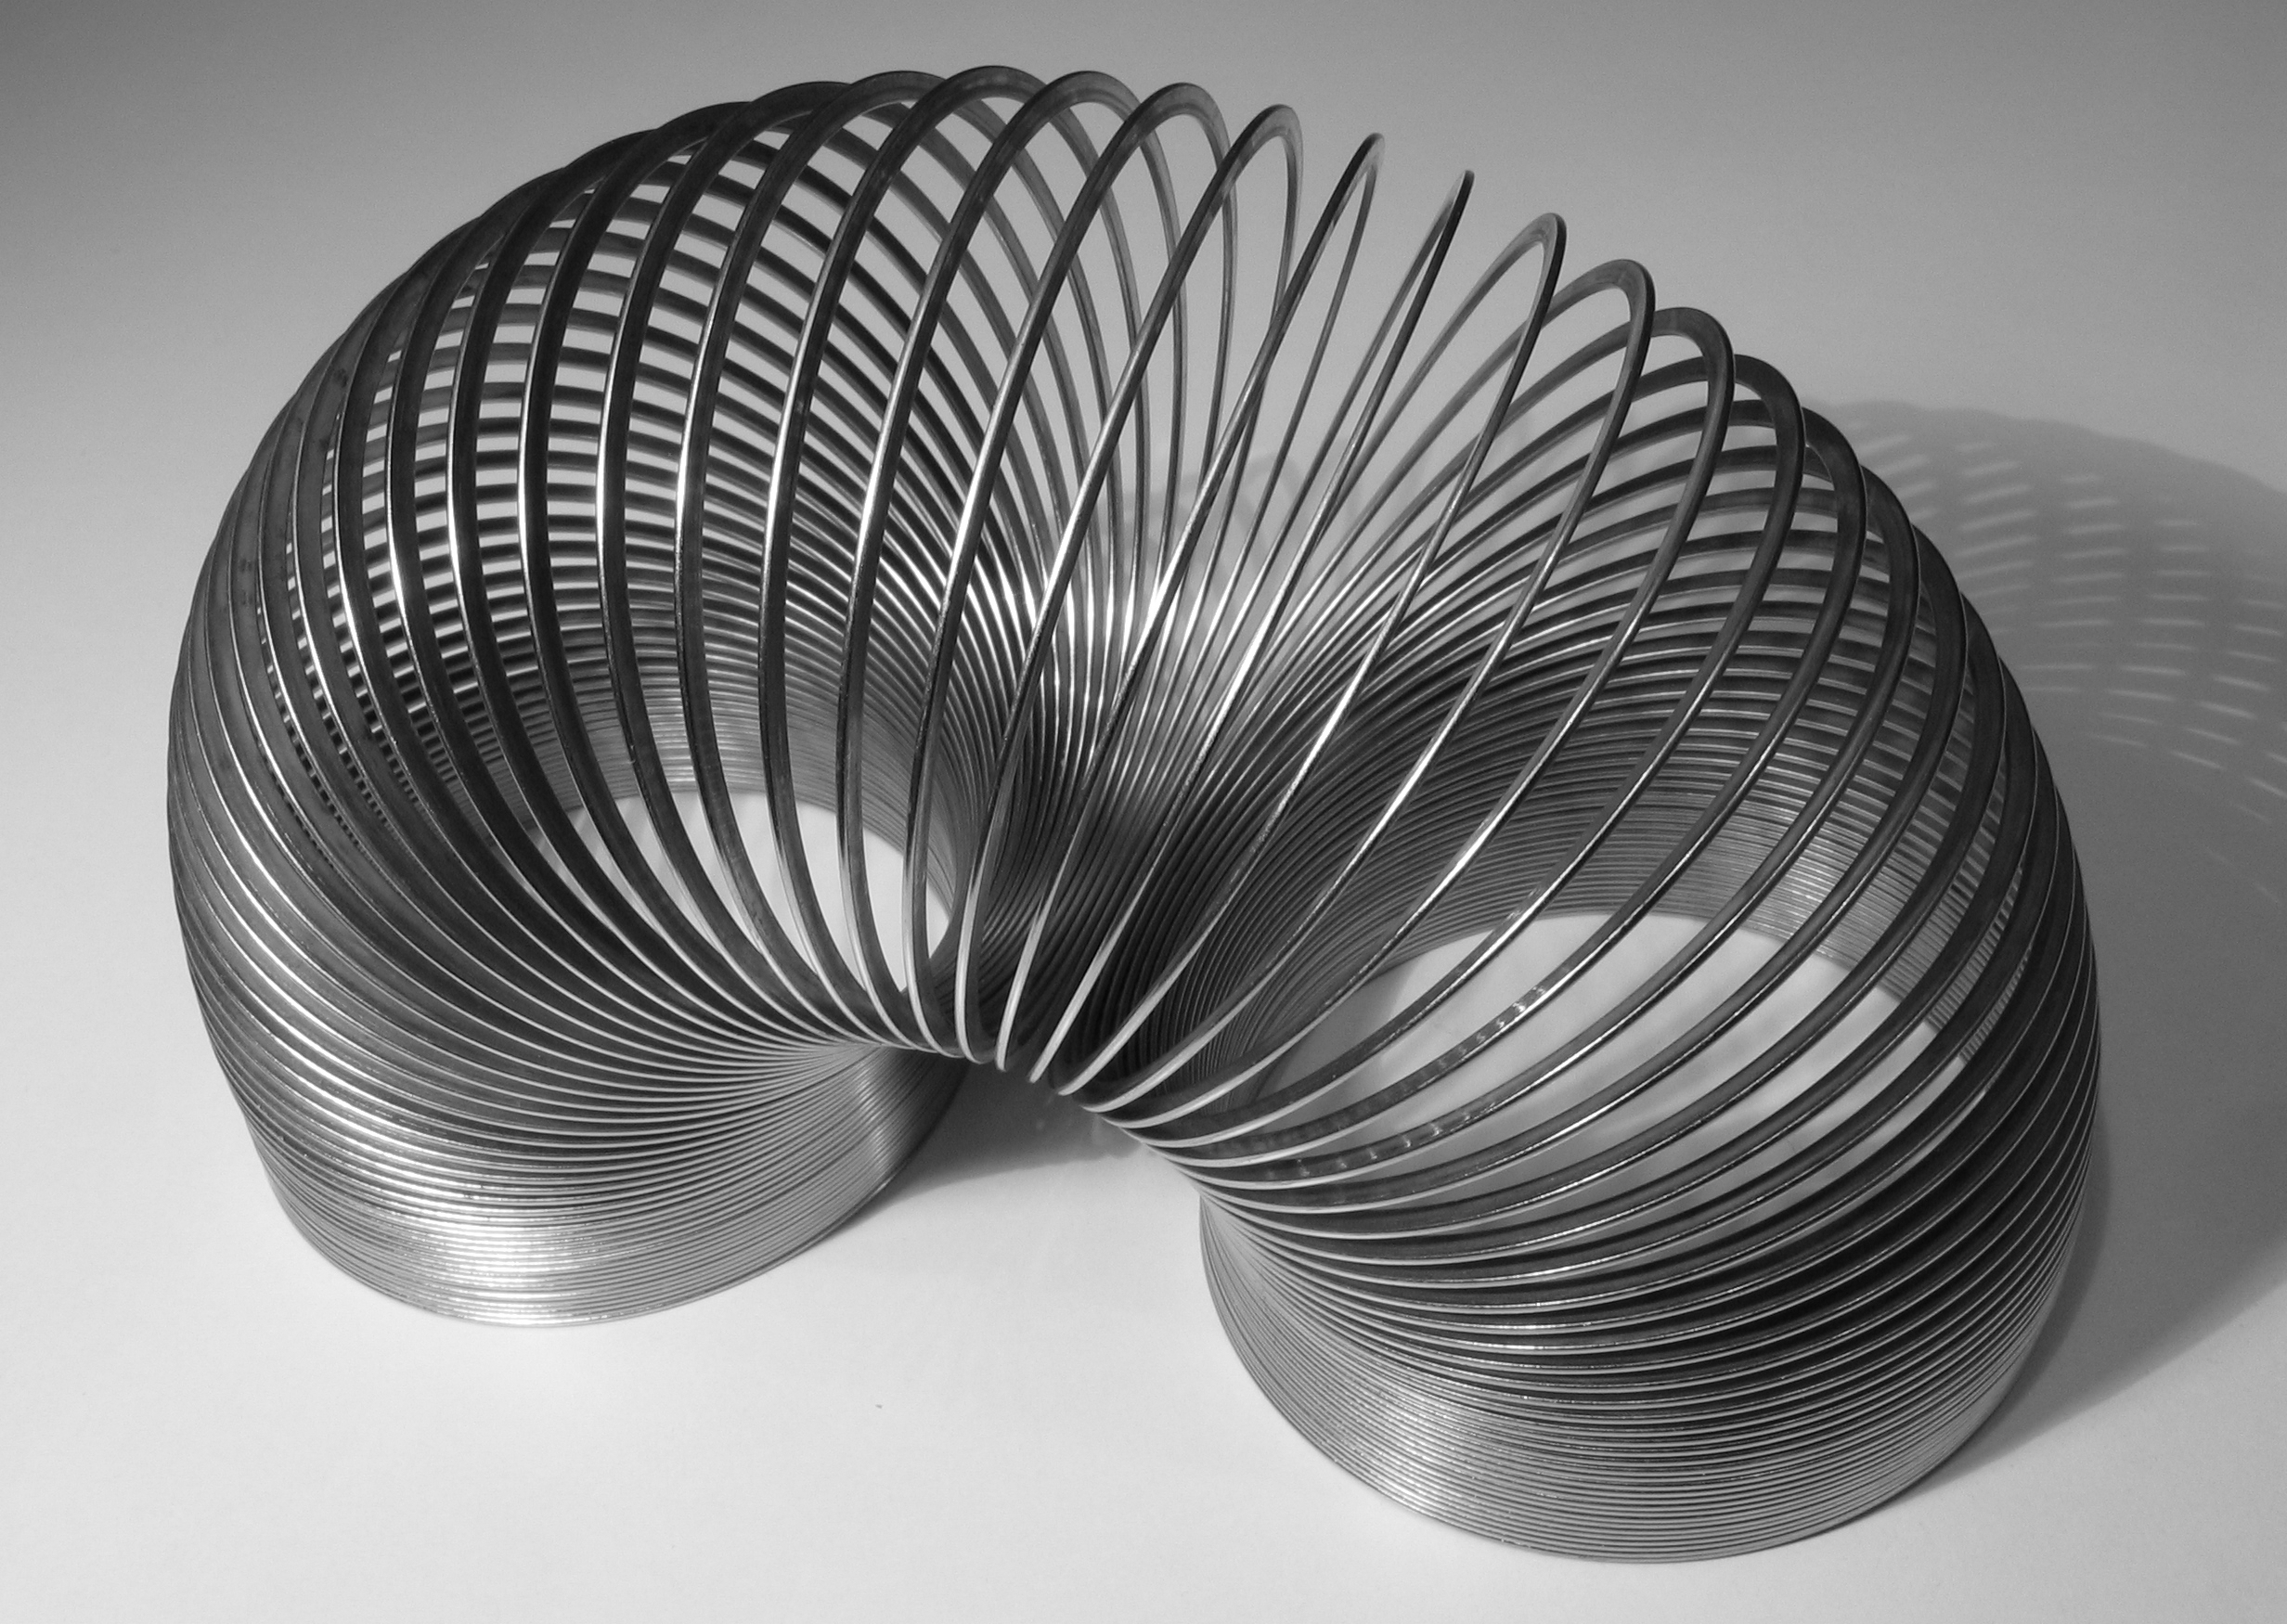
\includegraphics[width=0.45\textwidth]{slinky.jpg}
\quad

\includegraphics[width=0.45\textwidth]{guitar.jpg}
\end{center}

\section{Linear operators, revisited}

\index{linear operator}

Okay, so what does all this have to do with linear algebra? Well, consider the
linear operators we learned about in Section~\ref{linearOps}
(p.~\pageref{linearOps}). Remember that a linear operator is a square matrix
that transforms one vector into another one of the same dimension when you
left-multiply that vector by the matrix. Let's look at this one:


\begin{align*}
\renewcommand*{\arraystretch}{1.4}
M =
\begin{bmatrix}
1\frac{1}{2} & -1 \\
\smallskip
-\frac{1}{2} & 1 \\
\end{bmatrix},
\end{align*}

\label{mmatrix}

and take it for a spin. If we multiply it by, say, {\footnotesize $\begin{bmatrix} 1
\\ 2 \end{bmatrix}$}, we get:

\begin{align*}
\renewcommand*{\arraystretch}{1.4}
\small
\begin{bmatrix}
1\frac{1}{2} & -1 \\
\smallskip
-\frac{1}{2} & 1 \\
\end{bmatrix} \cdot
\begin{bmatrix}
1 \\ 2 \\
\end{bmatrix} =
\begin{bmatrix}
-\frac{1}{2} \\ 1\frac{1}{2} \\
\end{bmatrix}, \normalsize \quad \textrm{so}\
\boldmath
\begin{bmatrix}
1 \\ 2 \\
\end{bmatrix} \rightarrow \textrm{\textbf{\footnotesize maps to}} \rightarrow
\begin{bmatrix}
-\frac{1}{2} \\ 1\frac{1}{2} \\
\end{bmatrix}.
\unboldmath
\end{align*}

\label{thatExample}
For the input {\footnotesize $\begin{bmatrix} 2 \\ 1 \end{bmatrix}$}, we get:

\vspace{-.2in}
\begin{align*}
\renewcommand*{\arraystretch}{1.4}
\small
\begin{bmatrix}
1\frac{1}{2} & -1 \\
\smallskip
-\frac{1}{2} & 1 \\
\end{bmatrix} \cdot
\begin{bmatrix}
2 \\ 1 \\
\end{bmatrix} =
\begin{bmatrix}
2 \\ 0 \\
\end{bmatrix}, \normalsize \quad \textrm{so}\
\boldmath
\begin{bmatrix}
2 \\ 1 \\
\end{bmatrix} \rightarrow
\begin{bmatrix}
2 \\ 0 \\
\end{bmatrix}.
\unboldmath
\end{align*}

And $M$ maps the input {\footnotesize $\begin{bmatrix} -3 \\ 5 \end{bmatrix}$} to:

\vspace{-.2in}
\begin{align*}
\renewcommand*{\arraystretch}{1.4}
\small
\begin{bmatrix}
1\frac{1}{2} & -1 \\
\smallskip
-\frac{1}{2} & 1 \\
\end{bmatrix} \cdot
\begin{bmatrix}
-3 \\ 5 \\
\end{bmatrix} =
\begin{bmatrix}
-9\frac{1}{2} \\ 6\frac{1}{2} \\
\end{bmatrix}, \normalsize \quad \textrm{so}\
\boldmath
\begin{bmatrix}
-3 \\ 5 \\
\end{bmatrix} \rightarrow
\begin{bmatrix}
-9\frac{1}{2} \\ 6\frac{1}{2} \\
\end{bmatrix}.
\unboldmath
\end{align*}

See a pattern? Me neither. It seems to be all over the place, mapping each
input to some random output with no real rhyme or reason. All of these mappings
are depicted in Figure~\ref{nonEigenvec} (p.~\pageref{nonEigenvec}).

\begin{figure}[ht]
\centering
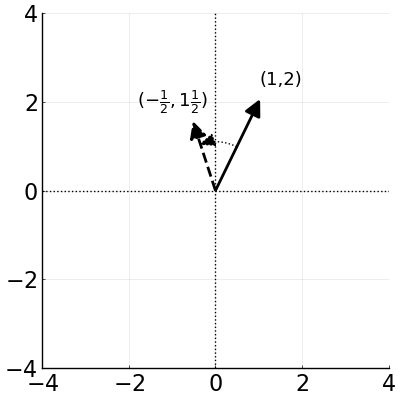
\includegraphics[width=0.4\textwidth]{crazytrans1.png} \quad
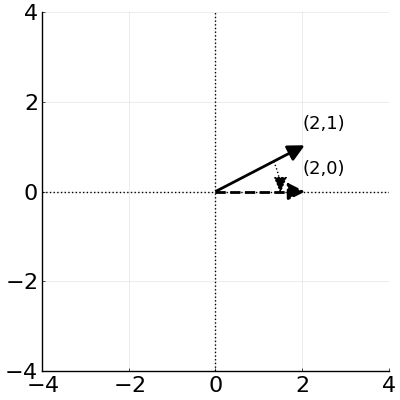
\includegraphics[width=0.4\textwidth]{crazytrans2.png} \\
\smallskip
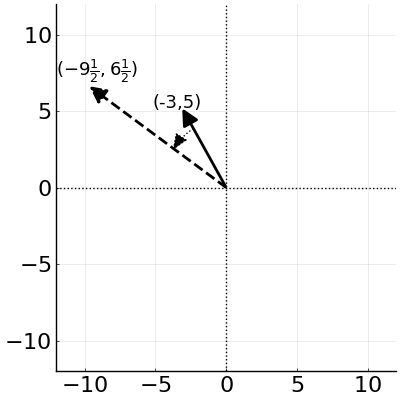
\includegraphics[width=0.4\textwidth]{crazytrans3.png}
\caption{The $M$ matrix's operation. Three randomly-chosen input vectors
(solid) are mapped to crazy output vectors (dashed).}
\label{nonEigenvec}
\end{figure}


\subsection{Hitting a matrix's resonant frequency}

None of that was very special. Random-looking stuff gets mapped to other
random-looking stuff. But now here comes the plot twist. Let's strike this bad
boy at its \textit{resonant frequency}.

% [ 1 1 ], [ -2 1 ]

\vspace{-.2in}
\begin{align*}
\renewcommand*{\arraystretch}{1.4}
\small
\begin{bmatrix}
1\frac{1}{2} & -1 \\
\smallskip
-\frac{1}{2} & 1 \\
\end{bmatrix} \cdot
\begin{bmatrix}
-1 \\ \frac{1}{2} \\
\end{bmatrix} =
\begin{bmatrix}
-2 \\ 1 \\
\end{bmatrix}, \normalsize \quad \textrm{so}\
\boldmath
\begin{bmatrix}
-1 \\ \frac{1}{2} \\
\end{bmatrix} \rightarrow
\begin{bmatrix}
-2 \\ 1 \\
\end{bmatrix}.
\unboldmath
\end{align*}

It's easy to miss the significance of that, so if nothing jumped out at you,
look again. What we just discovered is that the vector {\footnotesize
$\begin{bmatrix} -1 \\ \frac{1}{2} \end{bmatrix}$} is sort of magic: if we feed
it as input to $M$, the output is \textit{a scaled version of the same vector}.
In fact, it exactly doubled in size.

\smallskip

Let's try that again, with the {\footnotesize $\begin{bmatrix} -2 \\ 1
\end{bmatrix}$} we just got back:

\vspace{-.2in}
\begin{align*}
\renewcommand*{\arraystretch}{1.4}
\small
\begin{bmatrix}
1\frac{1}{2} & -1 \\
\smallskip
-\frac{1}{2} & 1 \\
\end{bmatrix} \cdot
\begin{bmatrix}
-2 \\ 1 \\
\end{bmatrix} =
\begin{bmatrix}
-4 \\ 2 \\
\end{bmatrix}, \normalsize \quad \textrm{so}\
\boldmath
\begin{bmatrix}
-2 \\ 1 \\
\end{bmatrix} \rightarrow
\begin{bmatrix}
-4 \\ 2 \\
\end{bmatrix}.
\unboldmath
\end{align*}

Boom. It exactly doubled again. And if we then feed it {\footnotesize
$\begin{bmatrix} -4 \\ 2 \end{bmatrix}$}:

\vspace{-.2in}
\begin{align*}
\renewcommand*{\arraystretch}{1.4}
\small
\begin{bmatrix}
1\frac{1}{2} & -1 \\
\smallskip
-\frac{1}{2} & 1 \\
\end{bmatrix} \cdot
\begin{bmatrix}
-4 \\ 2 \\
\end{bmatrix} =
\begin{bmatrix}
-8 \\ 4 \\
\end{bmatrix}, \normalsize \quad \textrm{so}\
\boldmath
\begin{bmatrix}
-4 \\ 2 \\
\end{bmatrix} \rightarrow
\begin{bmatrix}
-8 \\ 4 \\
\end{bmatrix}.
\unboldmath
\end{align*}

\index{piano}
\index{middle C}

Boom. It exactly doubled again. This is very intriguing. Vectors in this one
particular direction aren't ``jumping around'' like the other ones did when $M$
acted on them. Instead, the matrix just plays them back for us (at twice the
volume) like a pure middle C singing out from a piano. Figure~\ref{eigenvec1}
%(p.~\pageref{eigenvec1})
shows the illustration.

\begin{figure}[ht]
\centering
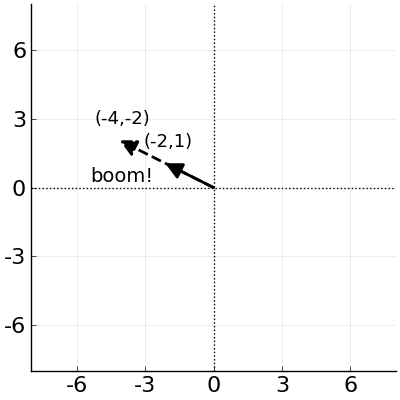
\includegraphics[width=0.4\textwidth]{eigentrans1.png} \quad
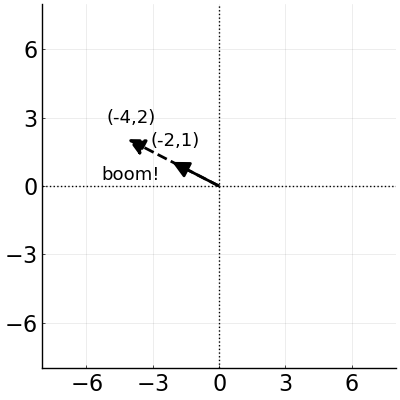
\includegraphics[width=0.4\textwidth]{eigentrans2.png} \\
\smallskip
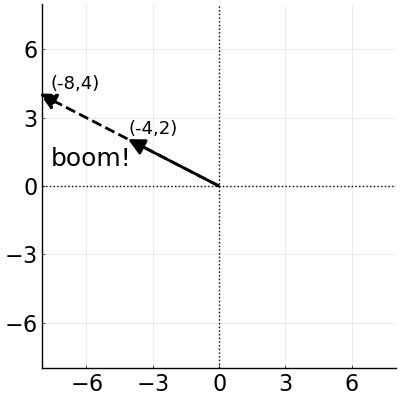
\includegraphics[width=0.4\textwidth]{eigentrans3.png}
\caption{The $M$ matrix's operation when applied to one of its eigenvectors.
The input (solid) is mapped to the \textit{same} vector, but scaled (dashed).}
\label{eigenvec1}
\end{figure}

\pagebreak
\index{eigenvector}
\index{eigenvalue}

Big concept: the vector {\footnotesize $\begin{bmatrix} -1 \\ \frac{1}{2}
\end{bmatrix}$} (and all its multiples, like {\footnotesize $\begin{bmatrix} -2
\\ 1 \end{bmatrix}$}, {\footnotesize $\begin{bmatrix} -4 \\ 2 \end{bmatrix}$},
{\footnotesize $\begin{bmatrix} -8 \\ 4 \end{bmatrix}$},
$\dots$) is called an \textbf{eigenvector} of $M$. Here's what that means:

\begin{framed}

An \textbf{eigenvector} of a matrix $A$ is any vector that gets mapped to a
scaled version of \textit{itself} -- \textit{i.e.}, to a vector in the same
direction -- when muliplied by $A$. In symbols, if
$\overrightarrow{\textbf{x}}$ is an eigenvector of $A$, then

{\centering
$ \displaystyle
A \overrightarrow{\textbf{x}} = \lambda \overrightarrow{\textbf{x}}$ \\
}

for some number $\lambda$. And that number $\lambda$ is called an
\textbf{eigenvalue} of $A$.
\end{framed}

In this case, the eigenvalue $\lambda$ is 2, since any vector in the
{\footnotesize $\begin{bmatrix} -1 \\ \frac{1}{2} \end{bmatrix}$} direction
gets multiplied by 2.

\subsection{Alternate resonant frequencies}

You might be curious: are there any \textit{other} ``magic'' vectors for our
$M$ matrix? It turns out there are. Try {\footnotesize $\begin{bmatrix} 4 \\ 4
\end{bmatrix}$}:

\vspace{-.2in}
\begin{align*}
\renewcommand*{\arraystretch}{1.4}
\small
\begin{bmatrix}
1\frac{1}{2} & -1 \\
\smallskip
-\frac{1}{2} & 1 \\
\end{bmatrix} \cdot
\begin{bmatrix}
4 \\ 4 \\
\end{bmatrix} =
\begin{bmatrix}
2 \\ 2 \\
\end{bmatrix}, \normalsize \quad \textrm{so}\
\boldmath
\begin{bmatrix}
4 \\ 4 \\
\end{bmatrix} \rightarrow
\begin{bmatrix}
2 \\ 2 \\
\end{bmatrix}.
\unboldmath
\end{align*}

So giving {\footnotesize $\begin{bmatrix} 4 \\ 4 \end{bmatrix}$} to the $M$
linear operator produces a \textit{shrunken} version of the input: exactly half
as long. And of course this pattern repeats for any vector in the
{\footnotesize $\begin{bmatrix} 4 \\ 4 \end{bmatrix}$} direction:

\vspace{-.2in}
\begin{align*}
\renewcommand*{\arraystretch}{1.4}
\small
\begin{bmatrix}
1\frac{1}{2} & -1 \\
\smallskip
-\frac{1}{2} & 1 \\
\end{bmatrix} \cdot
\begin{bmatrix}
2 \\ 2 \\
\end{bmatrix} =
\begin{bmatrix}
1 \\ 1 \\
\end{bmatrix}, \normalsize \quad \textrm{so}\
\boldmath
\begin{bmatrix}
2 \\ 2 \\
\end{bmatrix} \rightarrow
\begin{bmatrix}
1 \\ 1 \\
\end{bmatrix},
\unboldmath
\end{align*}

and so forth. This means that {\footnotesize $\begin{bmatrix} 4 \\ 4
\end{bmatrix}$} (and every other vector in the same direction) is also an
eigenvector of $M$, this time with eigenvalue $\lambda=\frac{1}{2}$.

\bigskip

Wow, okay. And does $M$ have still other eigenvectors in store for us as well?
The somewhat surprising answer turns out to be \textbf{\textit{no}}. There's
only those two. This is an important fact we'll return to in a moment.

\medskip

\index{dominant eigenvector}

To recap, then, our matrix $M$ has two eigenvectors: {\scriptsize
$\begin{bmatrix} -1 \\ \frac{1}{2} \end{bmatrix}$} (and any multiple of it) and
{\scriptsize $\begin{bmatrix} 4 \\ 4 \end{bmatrix}$} (and any multiple of it).
The first of these has eigenvalue 2, and the second has eigenvalue
$\frac{1}{2}$. Also, we have a special name for the {\scriptsize
$\begin{bmatrix} -1 \\ \frac{1}{2} \end{bmatrix}$} vector: it's called the
\textbf{dominant eigenvector}, for reasons you'll see in a moment. A matrix's
dominant eigenvector is simply the eigenvector with the highest eigenvalue.

\subsection{Magnetic pull}

Now assuming you followed all that, this next thing is sure to absolutely blow
your mind. I know it did mine. I'm going to feed a \textit{random} vector in as
an input to our $M$ matrix, and then repeatedly put its output back in to $M$
and see where it goes. Remember that if I do this with an \textit{eigenvector},
I'll keep getting back progressively scaled copies of the input vector. But
let's see what happens when I pass in just an ordinary, non-special, non-eigen
vector.

I'll choose {\footnotesize $\begin{bmatrix} 1 \\ 2\frac{1}{2} \end{bmatrix}$}
just for giggles, and call it $\overrightarrow{\textbf{r}}$ for ``random.'' If
I keep multiplying $\overrightarrow{\textbf{r}}$ by $M$, here's what I get:

\vspace{-.2in}
\begin{align*}
\renewcommand*{\arraystretch}{1.4}
\small
\overrightarrow{\textbf{r}} &=
\boldmath
\begin{bmatrix}
1 \\ 2\frac{1}{2} \\
\end{bmatrix}, \quad \textrm{ \ding{182}} \\
\unboldmath
\begin{bmatrix}
1\frac{1}{2} & -1 \\
\smallskip
-\frac{1}{2} & 1 \\
\end{bmatrix} \cdot
\begin{bmatrix}
1 \\ 2\frac{1}{2} \\
\end{bmatrix} &=
\boldmath
\begin{bmatrix}
-1 \\ 2 \\
\end{bmatrix}, \quad \textrm{ \ding{183}} \\
\unboldmath
\begin{bmatrix}
1\frac{1}{2} & -1 \\
\smallskip
-\frac{1}{2} & 1 \\
\end{bmatrix} \cdot
\begin{bmatrix}
-1 \\ 2 \\
\end{bmatrix} &=
\boldmath
\begin{bmatrix}
-3\frac{1}{2} \\ 2\frac{1}{2} \\
\end{bmatrix}, \quad \textrm{ \ding{184}} \\
\unboldmath
\begin{bmatrix}
1\frac{1}{2} & -1 \\
\smallskip
-\frac{1}{2} & 1 \\
\end{bmatrix} \cdot
\begin{bmatrix}
-3\frac{1}{2} \\ 2\frac{1}{2} \\
\end{bmatrix} &=
\boldmath
\begin{bmatrix}
-7\frac{3}{4} \\ 4\frac{1}{4} \\
\end{bmatrix}... \quad \textrm{ \ding{185}} \\
\unboldmath
\end{align*}

You might ask ``what's the big deal?''~until you look at the upper left of
Figure~\ref{converge1}, where I've plotted this sequence of vectors with the
circled numbers \ding{182}, \ding{183}, \ding{184}, and \ding{185}. I've also
plotted \textit{the dominant eigenvector} (which was in the direction
{\footnotesize $\begin{bmatrix} -1 \\ \frac{1}{2} \end{bmatrix}$}, as you
recall) \textit{as a dotted line} on this plot. Look at what happens: every
time we multiply by $M$, that random old vector is pulled towards $M$'s
dominant eigenvector like a magnet! And incredibly, this happens with
\textit{any} vector I start with. The other panes of Figure~\ref{converge1}
shows what happens when I start with {\footnotesize $\begin{bmatrix} -2 \\ -1
\end{bmatrix}$}, {\footnotesize $\begin{bmatrix} -1 \\ -2 \end{bmatrix}$}, and
{\footnotesize $\begin{bmatrix} 2 \\ \frac{1}{2} \end{bmatrix}$}. Resonant
frequency indeed!

\label{magneticPull}

\begin{figure}[ht]
\centering
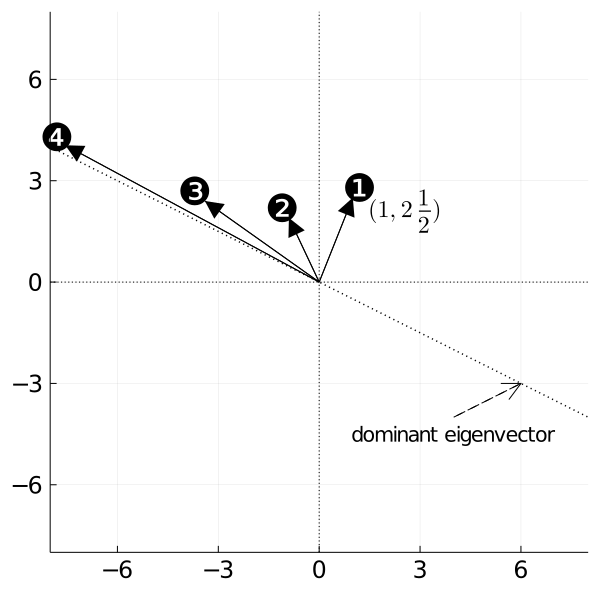
\includegraphics[width=0.4\textwidth]{converge1.png} \quad
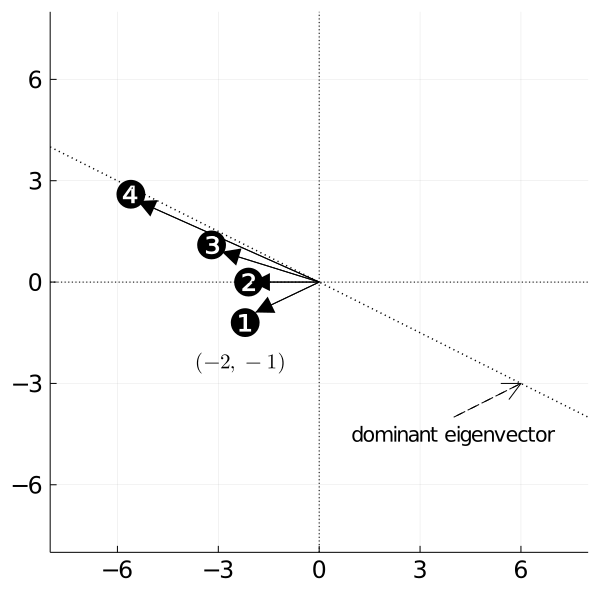
\includegraphics[width=0.4\textwidth]{converge2.png} \\
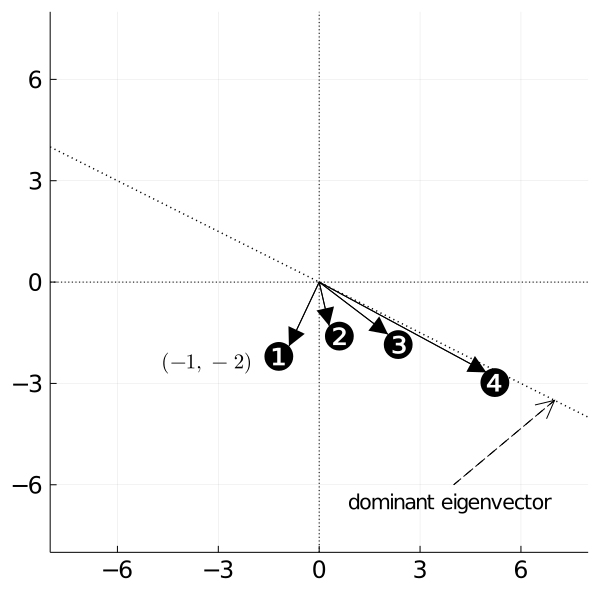
\includegraphics[width=0.4\textwidth]{converge3.png} \quad
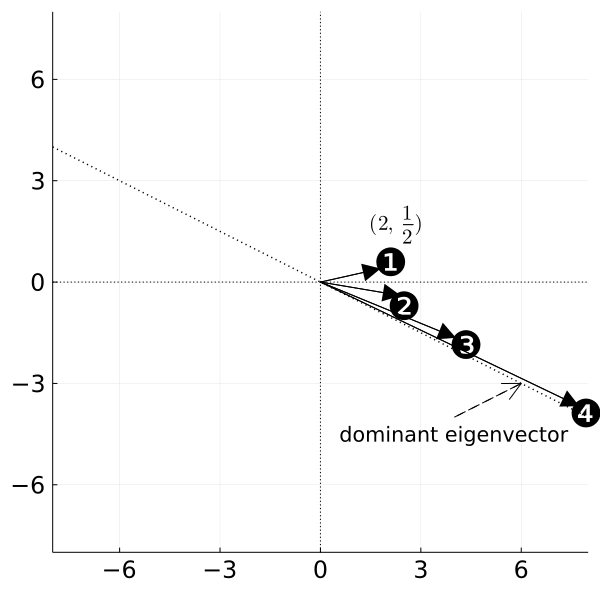
\includegraphics[width=0.4\textwidth]{converge4.png}
\caption{Holy cow -- repeatedly applying the $M$ operator by any vector at all
drags it progressively to the dominant eigenvector!}
\label{converge1}
\end{figure}

So we see that ``dominant'' eigenvector is an apt term. The matrix somehow
\textit{wants} to map its inputs to the direction of the dominant eigenvector.
If you keep multiplying by that matrix, you'll always be drawn there. And
that's true \textit{no matter what vector you started with.} This fact will
have immense repercussions when we look at things like Markov chains and the
PageRank algorithm in the next chapter.

In fact, the only vector I can start with and not get dragged to the dominant
eigenvector is one that is \textit{exactly} in the direction of the
\textit{other} eigenvector. As noted previously, if we give $M$ the input
{\footnotesize $\begin{bmatrix} 4 \\ 4 \end{bmatrix}$} (or anything in that
direction), it will stay locked in that direction (a 45\textdegree~angle
counterclockwise from the x-axis) and shrink by half each time. But if we nudge
that vector even slightly away from that other eigenvector -- say, to
{\scriptsize $\begin{bmatrix} 4 \\ 4.0001 \end{bmatrix}$} -- it'll get pulled
to the dominant eigenvector's direction ({\scriptsize $\begin{bmatrix} -1 \\
\frac{1}{2} \end{bmatrix}$}) instead.

\bigskip

In terms of our previous analogy, we're witnessing an even stronger sort of
``resonant frequency.'' With a playground swing, if we pump our legs at the
wrong pace, nothing much happens -- the swing just deadens. But imagine if
pumping our legs at the wrong pace got automatically \textit{converted} to the
right pace?

Or take another example. In real life, if an operatic soprano sings just the
right piercing note, she can shatter a nearby glass. But what if no matter what
note she sang, it was automatically adjusted by the glass to \textit{be} just
the perfect tone to shatter the glass? What we have here is not only a resonant
frequency, but a magnet pulling every vector \textit{towards} the resonant
frequency. Amazing.

\section{Basic principles}

All right, now let me give you the scoop. First, I'll tell you what's true
99.99\% of the time. Then, I'll say a few words about the other 0.01\%.

\index{scalar-vector multiplication}
\label{theScoopAboutEigenvectors}

In 99.99\% of cases, \textbf{an $n\times n$ matrix has $n$ different
eigenvectors.} Furthermore, each eigenvector will be linearly independent of
all the others. Each one has its own eigenvalue, and the eigenvector with the
highest eigenvalue is called the matrix's dominant eigenvector. This is exactly
what we saw with the $M$ matrix we've been using since p.~\pageref{mmatrix}: it
was $2\times 2$, and had two eigenvectors ({\scriptsize $\begin{bmatrix} -1 \\
\frac{1}{2} \end{bmatrix}$} and {\scriptsize $\begin{bmatrix} 4 \\ 4
\end{bmatrix}$}) with eigenvalues $\lambda=2$ and $\lambda=\frac{1}{2}$,
respectively. So {\scriptsize $\begin{bmatrix} -1 \\ \frac{1}{2}
\end{bmatrix}$} is the dominant one.\footnote{Note that when specifying the
eigenvectors, we could use \textit{any} vectors that point in the same
directions as these. For instance, it would also be correct to say that $M$'s
two eigenvectors are {\scriptsize $\begin{bmatrix} -2 \\ 1 \end{bmatrix}$} and
{\scriptsize $\begin{bmatrix} 1 \\ 1 \end{bmatrix}$}, or even {\scriptsize
$\begin{bmatrix} -50 \\ 25 \end{bmatrix}$} and {\scriptsize $\begin{bmatrix}
-1.73 \\ -1.73 \end{bmatrix}$}. Multiplying a vector by any constant, remember,
doesn't change its direction. And the eigen\textit{value} of a scaled
eigenvector doesn't change; the eigenvalues here are still 2 and $\frac{1}{2}$
no matter how we might scale the vectors.}

\smallskip

% This is old text: it turns out, as Dave M proved to Stephen on 10/13/2020,
% that singular matrices actually do have a full set of eigenvectors and do
% satisfy the spectral theorem.

%It's almost always this simple. The 0.01\% cases occur in one of two rare
%situations. One is when we're dealing with a blue matrix (\textit{i.e.}, a
%matrix whose columns are blue dominoes, \textit{i.e.}, a matrix some of whose
%columns are exact linear combinations of the others). As we've seen, blue
%matrices are strange and deficient and wreck all the rules, so this shouldn't
%surprise us. The good news is you're pretty unlikely to encounter a blue matrix
%out in the wild.
%
%The second rare case is

It's almost always this simple. The 0.01\% cases occur only in the weird
situation when we have a ``repeated eigenvalue'' and thus a ``duplicate
eigenvector.'' For example, the innocent-looking but ultimately weird matrix

\label{repeatedEigenvalue}
\vspace{-.25in}
\begin{align*}
W = \begin{bmatrix} -2 & 1 \\ -1 & 0 \end{bmatrix},
\end{align*}
\vspace{-.15in}

is an example of this. Its ``two eigenvectors'' turn out to be the
\textit{same}: {\scriptsize $\begin{bmatrix} 1 \\ 1 \end{bmatrix}$}. And each
one of them has eigenvalue -1. (Multiply out {\scriptsize $W\cdot
\begin{bmatrix} 1 \\ 1 \end{bmatrix}$} to verify that this produces
{\scriptsize $\begin{bmatrix} -1 \\ -1 \end{bmatrix}$}.) This scenario is 
very uncommon, and is unlikely to come up for you in practical situations.

%, and is akin to having a polynomial with a ``double root,'' as discussed
%below.

\smallskip

While you're building your understanding of this material, my advice is to
simply blow off the 0.01\% stuff. It's just a footnote. What's important is the
big takeaway: except in certain diabolically choreographed cases, the number of
eigenvectors is the width/height of the matrix, and each of them has its own
eigenvalue.

\subsection{Finding the eigenvectors/eigenvalues}

\label{eigenPython}
By the way, so far I've just stated to you what the eigenvectors are, and you
might wonder how I figured that out. The answer is that I simply gave the
matrix to Python and asked it for the eigenvectors and eigenvalues. We'll see
the code to do that at the end of the chapter. This is how you'll always do it
in practice.

%\smallskip
%\phantom{.}
%\pagebreak

\section{The Spectral Theorem}

\index{diagonalize (a matrix)}
\index{Spectral Theorem}
\label{SpectralTheorem}

And now I present to you a fundamental eigenvalue equation that has $E=mc^2$
level significance. It goes by several names: \textbf{The Spectral Theorem},
the \textbf{eigendecomposition}, and \textbf{diagonalizing} a matrix. It forms
the foundation of much of the advanced math that all this eigenstuff is based
on.

\smallskip
Here it is:
\vspace{-.15in}

\begin{framed}
\index{norm (of a vector)}

If $A$ is a $n\times n$ matrix, it can almost always\footnotemark~be decomposed
into the product of three other $n\times n$ matrices: $V\cdot \Lambda \cdot
V^{-1}$, where $V$ has the (normalized) eigenvectors of $A$ as its columns, and
$\Lambda$ is a diagonal matrix with the corresponding eigenvalues on the
diagonal. For example, for a $4\times 4$:

\vspace{-.15in}
\begin{align*}
A &=
\begin{bmatrix}
| & | & | & | \\[6pt]
\overrightarrow{\textbf{x}_{1}} &
\overrightarrow{\textbf{x}_{2}} &
\overrightarrow{\textbf{x}_{3}} &
\overrightarrow{\textbf{x}_{4}} \\
| & | & | & | \\[6pt]
\end{bmatrix} \
\begin{bmatrix}
\lambda_1 & 0 & 0 & 0 \\
0 & \lambda_2 & 0 & 0 \\
0 & 0 & \lambda_3 & 0 \\
0 & 0 & 0 & \lambda_4 \\
\end{bmatrix} \
\begin{bmatrix}
| & | & | & | \\[6pt]
\overrightarrow{\textbf{x}_{1}} &
\overrightarrow{\textbf{x}_{2}} &
\overrightarrow{\textbf{x}_{3}} &
\overrightarrow{\textbf{x}_{4}} \\
| & | & | & | \\[6pt]
\end{bmatrix}^{-1} \
\end{align*}
where the $\overrightarrow{\textbf{x}_k}$'s are the eigenvectors and the
$\lambda_k$'s are the corresponding eigenvalues.
%\vspace{-.15in}
\end{framed}

\footnotetext{99.99\% of the time. (See p.~\pageref{repeatedEigenvalue}.)}

\index{diagonalize (a matrix)}
\index{Spectral Theorem}
\index{eigendecomposition}

Terminology: decomposing a matrix $A$ into these three matrices -- the first of
which has the eigenvectors and the second of which has the eigenvalues -- is
called the \textbf{eigendecomposition} of the matrix. We also say that we have
``\textbf{diagonalized}'' $A$ because the middle matrix of the three (called
$\Lambda$, which is an upper case $\lambda$ ``lambda'') is a diagonal matrix.
Finally, this whole fact is also sometimes called \textbf{the Spectral Theorem}
for square matrices.

\subsection{Example}


Let's verify the Spectral Theorem for our $M$ matrix from p.~\pageref{mmatrix}.
I told you that the eigenvectors were {\footnotesize $\begin{bmatrix} -1 \\
\frac{1}{2} \end{bmatrix}$} and {\footnotesize $\begin{bmatrix} 4 \\ 4
\end{bmatrix}$}, but for the eigendecomposition we need them to have Euclidean
norm 1. So we normalize them (recall p.~\pageref{normalizing}) to get:

\index{normalizing (a vector)}

\vspace{-.15in}
\begin{align*}
\overrightarrow{x_1} =
\dfrac{\begin{bmatrix} -1 \\ \frac{1}{2} \end{bmatrix}}
{\left\lVert{\begin{bmatrix} -1 \\ \frac{1}{2} \end{bmatrix}}\right\rVert_2} =
\dfrac{\begin{bmatrix} -1 \\ \frac{1}{2} \end{bmatrix}}
{\sqrt{(-1)^2 + (\frac{1}{2})^2}} &=
\begin{bmatrix} -.894 \\ .447 \end{bmatrix}\\
\medskip\\
\overrightarrow{x_2} =
\dfrac{\begin{bmatrix} 4 \\ 4 \end{bmatrix}}
{\left\lVert{\begin{bmatrix} 4 \\ 4 \end{bmatrix}}\right\rVert_2} =
\dfrac{\begin{bmatrix} 4 \\ 4 \end{bmatrix}}
{\sqrt{(4)^2 + (4)^2}} &=
\begin{bmatrix} .707 \\ .707 \end{bmatrix}\\
\end{align*}
\vspace{-.25in}

It's important to note that these normalized versions of our eigenvectors point
in the \textit{same} directions that the original ones did ({\footnotesize
$\begin{bmatrix} -1 \\ \frac{1}{2} \end{bmatrix}$} and {\footnotesize
$\begin{bmatrix} 4 \\ 4 \end{bmatrix}$}). We just scaled them so that they have
length 1 (according to the Euclidean norm). But they're still the same
eigenvectors.

\medskip

Okay. Now if the Spectral Theorem is correct, $M$ should be equal to its
eigendecomposition. First, let's put together our $V$ matrix (with eigenvectors
as columns):

\label{mmatrixST}

\vspace{-.15in}
\begin{align*}
V =
\begin{bmatrix}
-.894 & .707 \\
.447 & .707 \\
\end{bmatrix}
\end{align*}
\vspace{-.15in}

Then, let's find its inverse (using Python):

\vspace{-.15in}
\begin{align*}
V^{-1} =
\begin{bmatrix}
-.746 & .746 \\
.471 & .943 \\
\end{bmatrix}
\end{align*}
\vspace{-.15in}

Next, stick the eigenvalues on the diagonal of an otherwise-all-zeroes matrix:

\vspace{-.15in}
\begin{align*}
\Lambda =
\begin{bmatrix}
2 & 0 \\
0 & \frac{1}{2} \\
\end{bmatrix}
\end{align*}
\vspace{-.15in}

and finally, multiply it all out:

\medskip
\begin{tabular}{CCCCCCC}
V & \cdot & \Lambda & \cdot & V^{-1} & = &M? \\
\smallskip \\
\begin{bmatrix}
-.894 & .707 \\
.447 & .707 \\
\end{bmatrix}
& \cdot &
\begin{bmatrix}
2 & 0 \\
0 & \frac{1}{2} \\
\end{bmatrix}
& \cdot &
\begin{bmatrix}
-.746 & .746 \\
.471 & .943 \\
\end{bmatrix}
& = &
\begin{bmatrix}
-1.5 & -1 \\
-.5 & 1 \\
\end{bmatrix}
\quad \checkmark
\end{tabular}
\smallskip

which indeed equals our $M$ from p.~\pageref{mmatrix}.

\section{The ``natural'' basis}

\index{Ron}
\index{Hermione}
\index{basis}

Now think back all the way to p.~\pageref{basis} when we talked about the
notion of a \textbf{basis}: a linearly independent set of vectors that spans
some space. You'll recall our friends Ron and Hermione, whose vectors
$\overrightarrow{\textbf{r}}$ and $\overrightarrow{\textbf{h}}$ we expressed in
both the standard basis $\{[\ 1\ \ 0\ ], [\ 0\ \ 1\ ]\}$, and in a ``domino
basis'' $\{[\ 1\ \ 2\ ], [\ 4\ \ 4\ ]\}$. Importantly, if you have a basis,
every vector in the space can be expressed as a linear combination of the basis
vectors in exactly one way.

\index{eigenbasis}

I'm now going to argue that in an important sense, the eigenvectors of a linear
operator matrix form the most ``natural'' basis for it. We call this set of
eigenvectors the \textbf{eigenbasis} of the matrix. Let me explain why it's the
most natural one.

First of all, realize that multiplying any matrix by a \textit{diagonal} one is
super easy. All you're doing is taking multiples of each column.

\pagebreak

\index{scattershot}

To illustrate, consider the following scattershot matrix, which I chose at
random and will call $S$:

\vspace{-.15in}
\begin{align*}
S = \begin{bmatrix}
3 & 4 & 2 & 1 \\
5 & 5 & -7 & 8 \\
1 & 1 & 1 & 2 \\
3 & 4 & 6 & 8 \\
\end{bmatrix}.
\end{align*}
\vspace{-.15in}

Now think about this. If I told you to multiply (by hand) $S$ times the matrix
below, you'd probably cry:

\vspace{-.15in}
\begin{align*}
\begin{bmatrix}
3 & 4 & 2 & 1 \\
5 & 5 & -7 & 8 \\
1 & 1 & 1 & 2 \\
3 & 4 & 6 & 8 \\
\end{bmatrix} \cdot
\begin{bmatrix}
3 & 2 & 1 & 9 \\
6 & 2 & -2 & 9 \\
1 & 9 & -3 & 9 \\
7 & 9 & 4 & 9 \\
\end{bmatrix} = \textbf{HARD} = \ ?? \ \frownie{}
\end{align*}
\vspace{-.05in}

But if I told you to compute \textit{this} operation by hand, you wouldn't cry:

\vspace{-.25in}
\begin{align*}
\begin{bmatrix}
3 & 4 & 2 & 1 \\
5 & 5 & -7 & 8 \\
1 & 1 & 1 & 2 \\
3 & 4 & 6 & 8 \\
\end{bmatrix} \cdot
\begin{bmatrix}
3 & 0 & 0 & 0 \\
0 & 2 & 0 & 0 \\
0 & 0 & -3 & 0 \\
0 & 0 & 0 & 9 \\
\end{bmatrix} = \textbf{easy!} =
\begin{bmatrix}
9 & 8 & -6 & 9 \\
15 & 10 & 21 & 72 \\
3 & 2 & -3 & 18 \\
9 & 8 & -18 & 72 \\
\end{bmatrix}\textrm{!}
\end{align*}
\vspace{-.15in}

The reason this operation is easy is that each column of the right-hand-side
matrix has all zero entries but one. Consider its first (leftmost) column, $[\
3\ \ 0\ \ 0\ \ 0\ ]^\intercal$. That says, ``for the first column of my answer,
I'd like three of $S$'s first column, and none of the others.'' So the first
column of our answer is simply $[\ 9\ \ 15\ \ 3\ \ 9\ ]^\intercal$: we just
multiply each entry by 3. Its second column is $[\ 0\ \ 2\ \ 0\ \ 0\
]^\intercal$, which means ``for the second column of my answer, I'd like two of
$S$'s second column, and none of the others.'' So the second column of the
answer is $[\ 8\ \ 10\ \ 2\ \ 8\ ]^\intercal$. And so on.

In fact, if you think of the columns of the $S$ matrix as a basis, the diagonal
matrix is doing nothing more than telling us \textit{how much of each basis
vector we want.} It's scaling each basis vector by a certain amount, and adding
them all together. And that's the key to seeing the eigenbasis'
``naturalness.''

\index{standard basis}
\index{change of basis}
\index{inverse}

Recall (from p.\pageref{changeOfBasisMatrix}) that if we have a vector
expressed in some basis $B$, and we want to convert it to the \textit{standard}
basis, we can multiply it by the appropriate change-of-basis matrix. And that
matrix simply has the basis vectors of $B$ as its columns.

Recall further (from p.\pageref{changeOfBasisOtherWayFinally}) that if we want
to go the other way -- if we have a vector expressed in the standard basis, and
we want to convert it to some other basis -- our change-of-basis matrix is the
\textit{inverse} of the one from the previous paragraph.

Now, let's put it all together. Suppose we wanted to take a linear operator $A$
for a test drive; that is, we want to multiply a square matrix $A$ by some
vector $\overrightarrow{\textbf{x}}$ to perform a linear transformation $A
\cdot \overrightarrow{\textbf{x}}$.

Look carefully at the spectral theorem formula again:

\vspace{-.15in}
\begin{align*}
A = V \cdot \Lambda \cdot V^{-1}.
\end{align*}
\vspace{-.15in}

This tells us that multiplying $\overrightarrow{\textbf{x}}$ by $A$ is the same
as multiplying it by those three matrices:

\vspace{-.15in}
\begin{align*}
A \cdot \overrightarrow{x} = V \cdot \Lambda \cdot V^{-1} \cdot
\overrightarrow{x}.
\end{align*}
\vspace{-.15in}

\index{associative (operation)}

Let's take these multiplications one at a time from the right.\footnote{We're
free to do it in this order if we want, because as you remember from
p.~\pageref{associative}, matrix multiplication is associative.} Consider what
each of them does:

\begin{compactenum}

\item Multiplying $\overrightarrow{x}$ by $V^{-1}$ converts
$\overrightarrow{x}$ from the standard basis to the eigenbasis. (!)

\item Then, multiplying by $\Lambda$ is a trivial operation which gives us ``a
certain amount'' of each eigenvector. (The ``amount'' is the eigenvalue
corresponding to that eigenvector, which effectively tells us how important
that eigenvector is to the result.)

\item Finally, multiplying $\overrightarrow{x}$ by $V$ converts
our answer from the eigenbasis back to the standard basis. (!)

\end{compactenum}

Dissected in this way, we get a super deep insight into what linear operators
fundamentally \textit{do}. Yes, you can think of them as matrix
multiplications. But under the hood, what we're really doing is converting our
input vector to a particular basis (the matrix's eigenbasis). Then, in that
space, ``matrix-vector multiplication'' is a simple scaling operation. We then
pop back into the standard basis for our final answer.

\smallskip

Just to make this concrete, let's work out an example using our $M$ matrix from
before (p.~\pageref{mmatrix}). From p.~\pageref{mmatrixST}, we learned that
$V$, the matrix with normalized eigenvectors as columns, was

\vspace{-.15in}
\begin{align*}
V = \begin{bmatrix}
-.894 & .707 \\
.447 & .707 \\
\end{bmatrix}.
\end{align*}
\vspace{-.15in}

As I explained above, this is really none other than the change-of-basis matrix
from $M$'s eigenbasis (we'll call that basis $B_\lambda$) to the standard basis
$B_s$. And if we take its inverse, we get the change-of-basis matrix going the
other way: from $B_s$ to $B_\lambda$. So,

\vspace{-.15in}
\begin{align*}
\textrm{COB}_{B_\lambda \rightarrow B_s} =
\begin{bmatrix}
-.894 & .707 \\
.447 & .707 \\
\end{bmatrix},\ 
\textrm{COB}_{B_s \rightarrow B_\lambda} =
\begin{bmatrix}
-.746 & .746 \\
.471 & .943 \\
\end{bmatrix}, 
\end{align*}
\vspace{-.15in}

where

\vspace{-.15in}
\begin{align*}
B_\lambda = \Bigg\{
\begin{bmatrix}
-.894 \\
.447 \\
\end{bmatrix}, 
\begin{bmatrix}
.707 \\
.707 \\
\end{bmatrix} \Bigg\}, \ \textrm{and}\ \ 
B_s = \Bigg\{
\begin{bmatrix}
1 \\
0 \\
\end{bmatrix}, 
\begin{bmatrix}
0 \\
1 \\
\end{bmatrix} \Bigg\}.
\end{align*}
\vspace{-.15in}

Now one of our example inputs to the $M$ linear transformation from
p.~\pageref{thatExample} was {\footnotesize $\begin{bmatrix} 2 \\ 1
\end{bmatrix}$}, which we saw $M$ map to {\footnotesize $\begin{bmatrix} 2 \\ 0
\end{bmatrix}$}. So let's run {\footnotesize $\begin{bmatrix} 2 \\ 1
\end{bmatrix}$} through the assembly line:

\smallskip
\begin{center}
\begin{tabular}{CCCCCCC}
\textrm{COB}_{B_\lambda \rightarrow B_s} & \cdot & \Lambda & \cdot &
\textrm{COB}_{B_s \rightarrow B_\lambda} & \cdot &
\begin{bmatrix} 2 \\ 1 \end{bmatrix}
\\
\\
\begin{bmatrix}
-.894 & .707 \\
.447 & .707 \\
\end{bmatrix}
& \cdot &
\begin{bmatrix}
2 & 0 \\
0 & \frac{1}{2} \\
\end{bmatrix}
& \cdot &
\begin{bmatrix}
-.746 & .746 \\
.471 & .943 \\
\end{bmatrix}
& \cdot &
\begin{bmatrix}
2 \\
1 \\
\end{bmatrix}
\end{tabular}
\end{center}
\smallskip

\begin{enumerate}
\itemsep1.5em

\item Multiplying our input vector {\footnotesize $\begin{bmatrix} 2 \\ 1
\end{bmatrix}$} -- whose coordinates are in the standard basis -- by $V^{-1}$
converts it to the eigenbasis.

\begin{center}
\begin{tabular}{CCCCC}
\textrm{COB}_{B_\lambda \rightarrow B_s} & \cdot & \Lambda & \cdot & \downarrow \\
\begin{bmatrix}
-.894 & .707 \\
.447 & .707 \\
\end{bmatrix}
& \cdot &
\begin{bmatrix}
2 & 0 \\
0 & \frac{1}{2} \\
\end{bmatrix}
& \cdot &
\begin{bmatrix}
-.746 \\
1.886 \\
\end{bmatrix}
\end{tabular}
\end{center}
\smallskip

So {\footnotesize $\begin{bmatrix} 2 \\ 1 \end{bmatrix}_{B_s}$} is the same as
{\footnotesize $\begin{bmatrix} -.746 \\ 1.886 \end{bmatrix}_{B_\lambda}$}, and
we're now in the ``eigenrealm,'' ready for the next step.

\item We now take that eigenbasis-version of our input and multiply it by
our diagonal matrix of eigenvalues.

\vspace{-.1in}
\begin{center}
\begin{tabular}{CCC}
\textrm{COB}_{B_\lambda \rightarrow B_s} & \cdot & \downarrow \\
\begin{bmatrix}
-.894 & .707 \\
.447 & .707 \\
\end{bmatrix}
& \cdot &
\begin{bmatrix}
-1.492 \\
.943 \\
\end{bmatrix}
\end{tabular}
\end{center}
\smallskip

We've merely scaled the eigenbasis-form of our input: the first element got
doubled from -.746 to -1.492 (since the first eigenvalue is 2) and the second
one got halved from 1.886 to .943 (since the second eigenvalue is
$\frac{1}{2}$). This was actually the only ``transformation'' work to do!

\item Now we merely translate our vector out of eigenspace back to standard
basis language, by multiplying by the change-of-basis matrix back the other way:

\vspace{-.15in}
\begin{align*}
& \ \downarrow \\
=
& \begin{bmatrix}
2 \\
0 \\
\end{bmatrix}\ !
\end{align*}
\vspace{-.15in}

Exactly as we predicted.

\end{enumerate}

\pagebreak

This is seriously one of the most beautiful things I've seen in all of
mathematics. It reminds me of an apple tree orchard. When you're wandering
through the grounds, it seems like you're in the middle of a chaotic maze of
trees planted in random positions. But when you happen upon a certain special
spot, boom! All the trees suddenly line up and a perfectly symmetric pattern
emerges. In a similar way, multiplying by a matrix looks like a jumble of
random numbers, but seen from one special perspective -- the eigenbasis -- the
operation suddenly becomes astonishingly simple and elegant.

\label{orchard}
\begin{center}
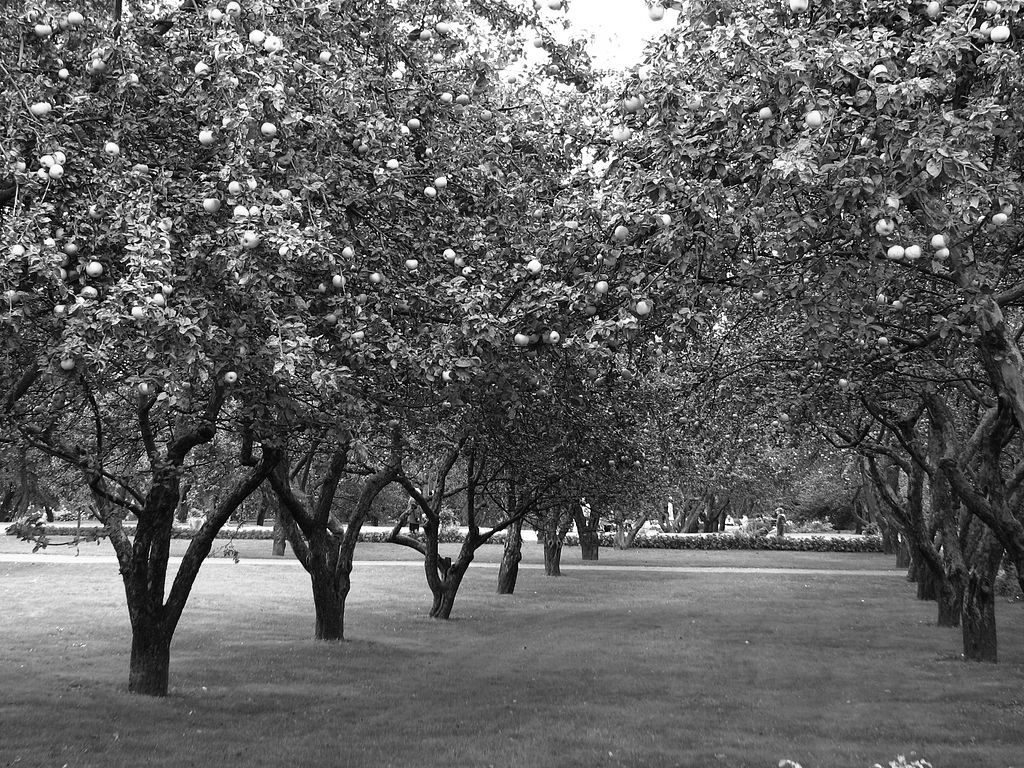
\includegraphics[width=0.8\textwidth]{orchard.jpg}
\end{center}

\subsection{Postlude: symmetric matrices and their eigenbases}

\index{symmetric matrix}
\index{orthonormal basis}
\index{covariance matrix}

One last little thing before we end this theoretical chapter and commence with
some exciting ``eigenapplications'' in the next one. It turns out that in many
situations, the square matrix $A$ that we're interested in will be
\textit{symmetric}. This is true if we're dealing with the adjacency matrix of
an undirected graph, for instance (recall the graph applications section
beginning on p.~\pageref{sec:graphs}). In statistical applications, we work
with something called a \textbf{covariance matrix} a lot, which shows how much
each pair of several random variables are correlated with each other. This,
too, will be a symmetric matrix.

\index{Spectral Theorem}

It turns out that the eigenvectors of a \textit{symmetric} matrix will always
form an \textbf{orthonormal basis}. This turns out to be convenient, because of
the lesson we learned on p.~\pageref{orthoInverseTranspose}: there we
discovered that if a matrix is orthogonal, its inverse is simply the same thing
as its transpose. And that means in turn that the Spectral Theorem for such
matrices reduces from this:

\begin{center}
$A = V\cdot \Lambda \cdot V^{-1}$
\end{center}

to simply this:

\begin{center}
$A = V\cdot \Lambda \cdot V^\intercal$.
\end{center}

The symmetric matrix $A$ itself is nothing more than its eigenvectors,
eigenvalues, and eigenvectors back-to-back-to-back.

Crisp and elegant, and as sweet smelling as an apple orchard. In our next and
final chapter, we'll eat a few of these juicy apples.

\vfill
\hrulefill \\

\pagebreak

\section*{\faPython \ \ \textit{Appendix: Python}}

On p.~\pageref{eigenPython} I mentioned that to actually find the eigenvalues
and eigenvectors of a matrix, you can just ask Python. Okay, so how do you do
that?

\index{linalg.eig@\texttt{linalg.eig()}}

Here's how: \texttt{linalg.eig()}. This function takes a matrix as an argument,
and returns a vector of two things: the eigenvalues (in their own vector), and
the corresponding eigenvectors. The latter come in a matrix where each column
is its own eigenvector, and where eigenvalue $k$ corresponds to the eigenvector
in column $k$.

Let's begin with the $M$ matrix (p.~\pageref{mmatrix}) we've been using all
chapter. I'll save the result from calling \texttt{linalg.eig()} (in a variable
called ``\texttt{eigstuff}'') and then print out each component separately.

\begin{Verbatim}[fontsize=\small,samepage=true,frame=single,framesep=3mm]
M = array([[1.5,-1],[-.5,1]])
eigstuff = linalg.eig(M)
print(eigstuff[0])
print(eigstuff[1])
\end{Verbatim}
\vspace{-.2in}

\begin{Verbatim}[fontsize=\small,samepage=true,frame=leftline,framesep=5mm,framerule=1mm]
[2.  0.5]
[[ 0.89442719  0.70710678]
 [-0.4472136   0.70710678]]
\end{Verbatim}

\index{normalizing (a vector)}

The two eigenvalues are 2 and $\frac{1}{2}$, as we knew. Now the numbers in the
eigenvector matrix look a little funky, but you just have to realize that
they've been normalized. That first eigenvector -- which goes with eigenvalue
2 -- is:

\begin{Verbatim}[fontsize=\small,samepage=true,frame=single,framesep=3mm]
dominant_eigvec = eigstuff[1][:,0]
print(dominant_eigvec)
\end{Verbatim}
\vspace{-.2in}

\begin{Verbatim}[fontsize=\small,samepage=true,frame=leftline,framesep=5mm,framerule=1mm]
[ 0.89442719 -0.4472136 ]
\end{Verbatim}

(Notice how I did that, by the way. I took \texttt{eigstuff}, accessed element
1 of it (the second element) to get the matrix of eigenvectors, and then used
``\texttt{:,0}'' in the boxies to get all rows of column 0.)

Now $[\ 0.894\ \ -0.447\ ]^\intercal$ may not look familiar, but remember that
it only indicates the \textit{direction} of the eigenvector. Any vector in the
same direction is also an eigenvector. So if we, say, divided it by the second
entry to get an equally good dominant eigenvector:

\begin{Verbatim}[fontsize=\small,samepage=true,frame=single,framesep=3mm]
another_eigvec = dominant_eigvec / dominant_eigvec[1]
print(another_eigvec)
\end{Verbatim}
\vspace{-.2in}

\begin{Verbatim}[fontsize=\small,samepage=true,frame=leftline,framesep=5mm,framerule=1mm]
[ -2. 1. ]
\end{Verbatim}

that should ring a bell. We can do the same with the other eigenvectors, of
course, and there's really nothing more to it than that. (Believe me:
calculating them by hand is a \textit{major} pain.)
